\documentclass[a4paper]{article}
\usepackage[utf8]{inputenc}
\usepackage{amsmath}
\usepackage[colorinlistoftodos]{todonotes}
\usepackage[utf8]{inputenc}
\usepackage{graphicx}
\graphicspath{ {figures/} }
\usepackage{array}
\usepackage{placeins}
\usepackage[left=0.5 in,top=0.5in,right=0.5 in,bottom=0.5in]{geometry}
\PassOptionsToPackage{hyphens}{url}
\usepackage{hyperref}
\usepackage{parskip}
\usepackage [english]{babel}
\usepackage [autostyle, english = american]{csquotes}
\MakeOuterQuote{"}
\hypersetup{
     colorlinks,
     urlcolor    = blue
}
\usepackage{xcolor}
\usepackage{listings}
\lstloadlanguages{Python}
\newcommand{\inlinecode}[1]{\lstinline{#1}}

\lstset{
  language=Python,
  basicstyle=\scriptsize\sffamily,
  numberstyle=\color{gray},
  stringstyle=\color[HTML]{933797},
  commentstyle=\color[HTML]{228B22}\sffamily,
  emph={[2]from,import,pass,return}, emphstyle={[2]\color[HTML]{DD52F0}},
  emph={[3]range}, emphstyle={[3]\color[HTML]{D17032}},
  emph={[4]for,in,def}, emphstyle={[4]\color{blue}},
  showstringspaces=false,
  breaklines=true,
  prebreak=\mbox{{\color{gray}\tiny$\searrow$}},
  numbers=left,
  xleftmargin=15pt
}

\title{Application 2: Analysis of a Computer Network \\Algorithmic Thinking (Part1)}
\author{Shamsuddin Rehmani}
\begin{document}
\sloppy
\maketitle
\section*{Application 2 Description}
Graph exploration (that is, "visiting" the nodes and edges of a graph) is a powerful and necessary tool to elucidate properties of graphs and quantify statistics on them. For example, by exploring a graph, we can compute its degree distribution, pairwise distances among nodes, its connected components, and centrality measures of its nodes and edges. As we saw in the Homework and Project, breadth-first search can be used to compute the connected components of a graph.

In this Application, we will analyze the connectivity of a computer network as it undergoes a cyber-attack. In particular, we will simulate an attack on this network in which an increasing number of servers are disabled. In computational terms, we will model the network by an undirected graph and repeatedly delete nodes from this graph. We will then measure the resilience of the graph in terms of the size of the largest remaining connected component as a function of the number of nodes deleted.

\section*{Answer to Question 1}
Probability p such that the ER graph computed using this edge probability has approximately the same number of edges as the computer network is 0.00397

Integer m such that the number of edges in the UPA graph is close to the number of edges in the computer network is 2

\FloatBarrier
% trim=l b r t
\begin{figure}[h]
	\centering 
	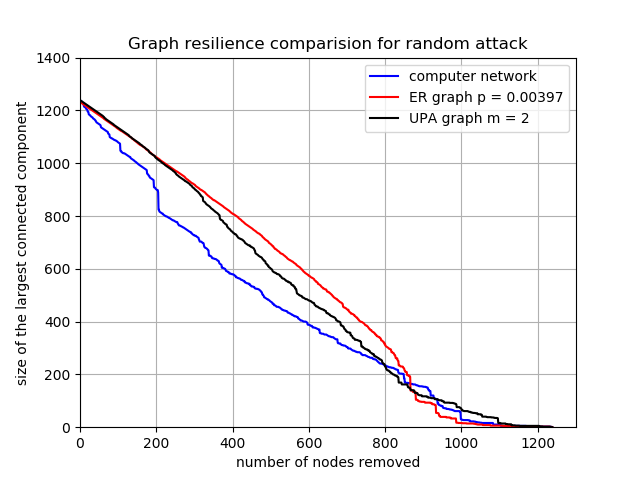
\includegraphics[scale = 0.9, clip=True, trim=0cm 0cm 0cm 0cm]{Q1_graph_resilience_comparision.png}
	\caption{graph resilience comparision for random attack for computer network, undirected ER graph, and UPA graph}
\end{figure}
\FloatBarrier

\newpage
\section*{Answer to Question 2}
All 3 graphs seem to be resilient (as shown in Figure 1), i.e the size of the largest connected component is within 25\% of 1000 (the approximate number of remaing nodes)


\section*{Answer to Question 3}

Big-O bounds for \texttt{target\char`_order} $= O(n^2 + m) = O(n^2)$ since for UPA graph $m <= 5n$ ($m = $ total 
number of edges in UPA)

Big-O bounds for \texttt{fast\char`_target\char`_order} $= O(n + m) = O(n)$ since for UPA graph $m <= 5n$ ($m = $ total number of edges in UPA)

\FloatBarrier
% trim=l b r t
\begin{figure}[h]
	\centering 
	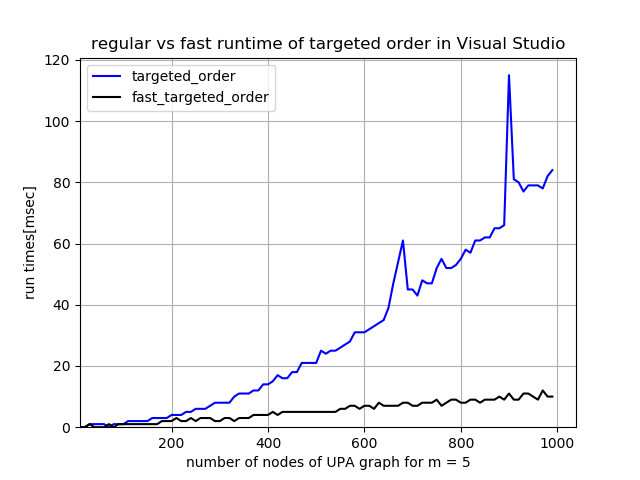
\includegraphics[scale = 1.0, clip=false, trim=0cm 0cm 0cm 0cm]{Q3_targeted_order_time_comparision.png}
	\caption{runtime for \texttt{target\char`_order} and \texttt{fast\char`_target\char`_order} on UPA graph with nodes ranging from 10 to 1000 for $m = 5$}
\end{figure}
\FloatBarrier

\newpage
\section*{Answer to Question 4}

\FloatBarrier
% trim=l b r t
\begin{figure}[h]
	\centering 
	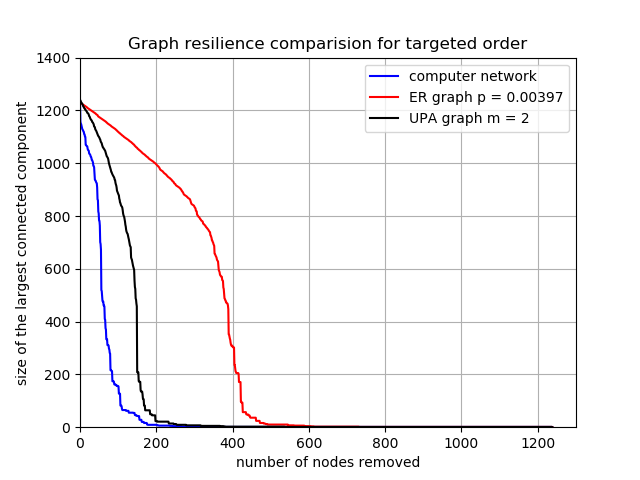
\includegraphics[scale = 1.0, clip=false, trim=0cm 0cm 0cm 0cm]{Q4_graph_resilience_comparision.png}
	\caption{graph resilience comparision for targeted attack for computer network, undirected ER graph, and UPA graph}
\end{figure}
\FloatBarrier

\section*{Answer to Question 5}
From the graph(Figure 3) we can see that only ER graph is resilient as the first 20\% of the nodes are removed while the UPA and the computer network graph reaches close to zero as 20\% of the ndoes are removed
 
\newpage

\appendix
\section{Python code used to answer the Application Questions}
\lstinputlisting{alg_application2_solution.py}
\section{All functions for project 4 used in the application}
\lstinputlisting{alg_project2_solution.py}
\section{Code for ER and UPA graph generations}
\lstinputlisting{alg_example_graphs.py}


\end{document}
